% !TEX TS-program = pdflatex
% !TEX encoding = UTF-8 Unicode

\documentclass[a4paper, titlepage=false, parskip=full-, 10pt]{scrartcl}

\usepackage[utf8]{inputenc}
\usepackage[T1]{fontenc}
\usepackage[english, ngerman]{babel}
\usepackage{babelbib}
\usepackage{hyperref}
\usepackage{listings}
\usepackage{framed}
\usepackage{color}
\usepackage{graphicx}
\usepackage[normalem]{ulem}
\usepackage{cancel}
\usepackage{amsmath}
\usepackage{amssymb}
\usepackage{amsthm}
\usepackage{algorithm}
\usepackage{algorithmic}
\usepackage{geometry}
\usepackage{subfigure}
\geometry{a4paper, top=20mm, left=35mm, right=25mm, bottom=40mm}

\newcounter{tasknbr}
\setcounter{tasknbr}{1}
\newenvironment{task}[1]{{\bf Aufgabe \arabic {tasknbr}\stepcounter{tasknbr}} (#1):\begin{enumerate}}{\end{enumerate}}
\newcommand{\subtask}[1]{\item[#1)]}

% Listings -----------------------------------------------------------------------------
\definecolor{red}{rgb}{.8,.1,.2}
\definecolor{blue}{rgb}{.2,.3,.7}
\definecolor{lightyellow}{rgb}{1.,1.,.97}
\definecolor{gray}{rgb}{.7,.7,.7}
\definecolor{darkgreen}{rgb}{0,.5,.1}
\definecolor{darkyellow}{rgb}{1.,.7,.3}
\lstloadlanguages{C++,[Objective]C,Java}
\lstset{
escapeinside={§§}{§§},
basicstyle=\ttfamily\footnotesize\mdseries,
columns=fullflexible,
keywordstyle=\bfseries\color{blue},
commentstyle=\color{darkgreen},      
stringstyle=\color{red},
numbers=left,
numberstyle=\ttfamily\scriptsize\color{gray},
breaklines=true,
showstringspaces=false,
tabsize=4,
captionpos=b,
float=htb,
frame=tb,
frameshape={RYR}{y}{y}{RYR},
rulecolor=\color{black},
xleftmargin=15pt,
xrightmargin=4pt,
aboveskip=\bigskipamount,
belowskip=\bigskipamount,
backgroundcolor=\color{lightyellow},
extendedchars=true,
belowcaptionskip=15pt}

%% Enter current values here: %%
\newcommand{\lecture}{Computer Vision WS15/16}
\newcommand{\tutor}{}
\newcommand{\assignmentnbr}{1}
\newcommand{\students}{Julius Auer}
\lstset{language=Octave}
%%-------------------------------------%%

\begin{document}  
{\small \textsl{\lecture \hfill \tutor}}
\hrule
\begin{center}
\textbf{Übungsblatt \assignmentnbr}\\
[\bigskipamount]
{\small \students}
\end{center}
\hrule

\begin{task}{Die Ersten Schritte}
\subtask{1.0}
\emph{Richte Dir eine geeignete Programmierumgebung ein. Ich empfehle Matlab oder Python.}

Für Bildbearbeitung im akademischen Kontext nehme ich gerne Octave - für Matlab-User sollte das ja auch lesbar sein.

\subtask{1.1}
\emph{Öffne das Testbild ''image.jpg'' (im Ressourcen-Bereich) und stelle es in einem Fenster dar.}

\begin{lstlisting}
img_ori = imread('image.jpg');
imshow(img_ori);
\end{lstlisting}

\subtask{1.2}
\emph{Extrahiere ein 60 x 60 Pixel großes Unterbild von Koordinate (50,110) und stelle es in einem Fenster dar.}

\begin{lstlisting}
img_pru = img_ori(50:110, 110:170, :);
\end{lstlisting}

\begin{figure}[htpb]
\begin{center}

\includegraphics[width=7cm]{image_pruned.jpg}
\end{center}
\caption{Pruned Image}
\end{figure}

\newpage
\subtask{1.3}
\emph{Stelle nur den Rotkanal dar.}

Die einfachste Möglichkeit dürfte sein, die rote Hyperebene als Grauwertbild zu interpretieren:

\begin{lstlisting}
img_red = img_ori(:, :, 1);
\end{lstlisting}

\begin{figure}[htpb]
\begin{center}
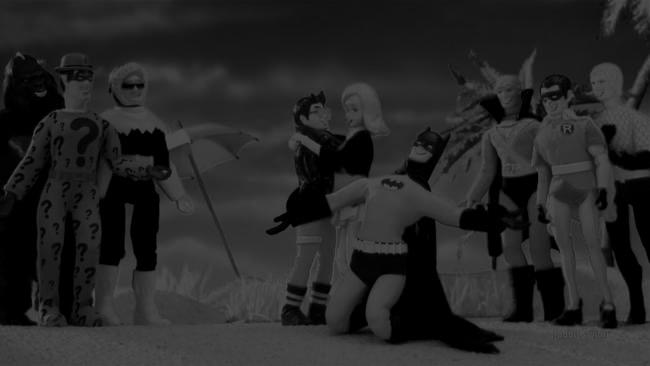
\includegraphics[width=9cm]{image_red.jpg}
\end{center}
\caption{Red-Only Image}
\end{figure}

\subtask{1.4}
\emph{Spiegele das Bild an der x-Achse und dann an der y-Achse.}

\begin{lstlisting}
img_fli_x   = img_ori(rows(img_ori):-1:1, :, :);
img_fli_y   = img_ori(:, columns(img_ori):-1:1, :);
\end{lstlisting}

\begin{figure}[htpb]
\begin{center}
\subfigure[Flip y]{
  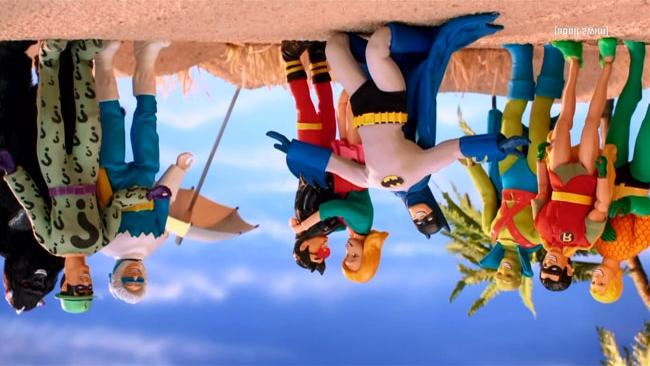
\includegraphics[width=7cm]{image_flip_x}
}
\subfigure[Flip x]{
  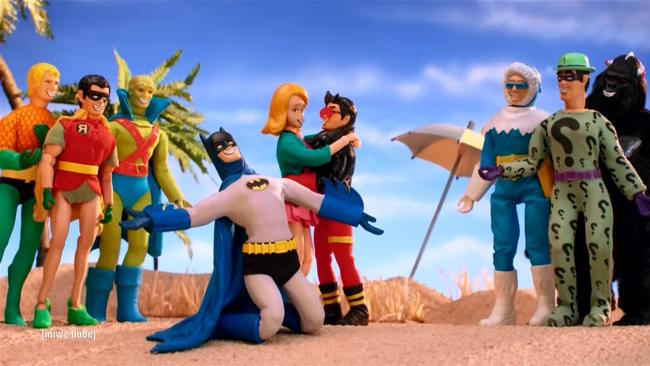
\includegraphics[width=7cm]{image_flip_y}
}
\end{center}
\caption{Flipped Images}
\end{figure}

\newpage
\subtask{1.5}
\emph{Wandle das Bild in ein Grauwertbild um und stelle es invertiert dar.}

Es gibt mit \emph{rgb2gray()} zwar auch einen Einzeiler für das Grauwertbild, ein kurzer Weg für das invertierte Bild ist mir jedoch nicht bekannt. Tja, dann muss ich hier wohl rechnen ... :

\begin{lstlisting}
img_gra_inv = uint8(255 - sum(img_ori, 3) / 3);
\end{lstlisting}

\begin{figure}[htpb]
\begin{center}
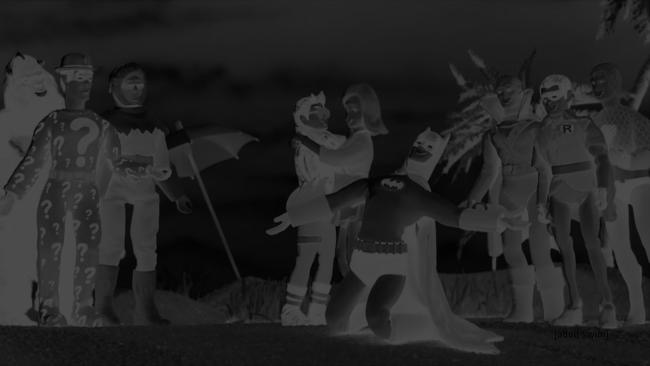
\includegraphics[width=9cm]{image_gray_inverted.jpg}
\end{center}
\caption{Inverted Grayscale Image}
\end{figure}
\end{task}

\begin{task}{Human vs. Computer Vision}
\item[]
\emph{Wie unterscheiden sich menschliches Auge und eine Kamera? Bitte in Stichpunkten antworten.}
\begin{table}[h]
\centering
\begin{tabular}{l|l}
Kamera	&	Auge\\\hline\hline
Variable Brennweite	&	Feste Brennweite\\\hline
Detektierbarer Bereich theoretisch fast beliebig	&	Detektierbarer Bereich ca. $380-780nm$\\\hline
Variable Belichtungszeit	&	Feste Belichtungszeit\\\hline
Anfällig für Motion-Blur	&	Robust gegen Motion-Blur\\\hline
Keine Tiefen-Wahrnehmung	&	3D\\\hline
Ggf. hohe Auflösung	&	''Nur'' ca. $3.4$ mPixel\\\hline
Ggf. hohe Sensibilität	&	Fester Treshold ab dem Alles schwarz
\end{tabular}
\caption{Auge vs. Kamera}
\end{table}
\end{task}

\begin{task}{Das invertierte After-Image}
\item[]
\emph{Warum nehmen wir nach Betrachtung der Beispielbilder (siehe Vorlesungsfolien) ein invertiertes Nachbild wahr? Die kürzeste, korrekte Erklärung wird prämiert!}

Ein den Wert $x$ perzeptionierendes Zäpfchen ''lernt'' bei Starren $x$, so dass bei anschließendem Blick auf eine weisse Fläche nur $255-x$ weitergeleitet wird.
\end{task}
\end{document}